\chapter{Specifikacija programske potpore}
		
			
		
	\section{Funkcionalni zahtjevi}
			
			
			%\textbf{\textit{dio 1. revizije}}\\
			
		%	\textit{Navesti \textbf{dionike} koji imaju \textbf{interes u ovom sustavu} ili  \textbf{su nositelji odgovornosti}. To su prije svega korisnici, ali i administratori sustava, naručitelji, razvojni tim.}\\
				
			%\textit{Navesti \textbf{aktore} koji izravno \textbf{koriste} ili \textbf{komuniciraju sa sustavom}. Oni mogu imati inicijatorsku ulogu, tj. započinju određene procese u sustavu ili samo sudioničku ulogu, tj. obavljaju određeni posao. Za svakog aktora navesti funkcionalne zahtjeve koji se na njega odnose.}\\
			
			
			\noindent \textbf{Dionici:}
			
			\begin{packed_enum}
				
				\item Posjetitelj
				\item Organizator			
				\item Administrator
				
			\end{packed_enum}
			
			\noindent \textbf{Aktori i njihovi funkcionalni zahtjevi:}
			
			
			\begin{packed_enum}
				\item  \underbar{Neregistrirani/neprijavljeni korisnik (inicijator) može:}
				
				\begin{packed_enum}
					
					\item pregled događanja
					\item odabir događanja i pregled općih informacija o događanju
					\item mogućnost registriranja kao posjetitelj, organizator ili administrator
					
				\end{packed_enum}
				
				\item  \underbar{Posjetitelj (inicijator) može:}
				
				\begin{packed_enum}
					
					\item pregled i mogućnost izmjene osobnih podataka
					\item brisanje vlastitog računa
					\item mogućnost ostavljanja recenzije na događaj
					\item mogućnost ostavljanja oznake zainteresiranosti za neki događaj
					\item mogućnost pretplaćivanja na obavijesti o budućim događanjima
					
					
				\end{packed_enum}
				
				\item  \underbar{Organizator (inicijator) može:}
				
				\begin{packed_enum}
									
					\item dodavanje događanja
					\item uređivanje informacija o svom događanju
					\item brisanje događanja
					\item obaveza plaćanja članarine ako se događanja naplaćuju
					
					
				\end{packed_enum}
				
				\item  \underbar{Administrator (inicijator) može:}
				
				\begin{packed_enum}	
					
					\item  pregled svih registriranih korisnika i njihovih osobnih podataka
					\item  brisanje i mijenjanje uloga korisnika
					\item  pristup statistici događanja i korisnika
					\item  brisanje recenzija koje krše pravila korištenja
					\item  postavljanje cijene članarina organizatora
					
				\end{packed_enum}
			
				\item  \underbar{Baza podataka (sudionik) može:}
				
				\begin{packed_enum}
					
					\item pohranjuje sve podatke o korisnicima i njihovim ovlastima
					\item pohranjuje sve podatke o događanjima
					
				\end{packed_enum}
				
				\item  \underbar{Banka (sudionik) može:}
				
				\begin{packed_enum}
					
					\item pruža uslugu plaćanja članarine
					
				\end{packed_enum}
				
				\item  \underbar{Paypal (sudionik) može:}
				
				\begin{packed_enum}
					
					\item pruža uslugu plaćanja članarine
					
				\end{packed_enum}
			\end{packed_enum}
			
			\eject 
			
			
				
			\subsection{Obrasci uporabe}
				
				%\textbf{\textit{dio 1. revizije}}
				
				\subsubsection{Opis obrazaca uporabe}
					%\textit{Funkcionalne zahtjeve razraditi u obliku obrazaca uporabe. Svaki obrazac je potrebno razraditi prema donjem predlošku. Ukoliko u nekom koraku može doći do odstupanja, potrebno je to odstupanje opisati i po mogućnosti ponuditi rješenje kojim bi se tijek obrasca vratio na osnovni tijek.}\\
					

					\noindent \underbar{\textbf{UC1 -Pregled događanja}}
					\begin{packed_item}
	
						\item \textbf{Glavni sudionik: }Korisnik, posjetitelj
						\item  \textbf{Cilj:} Pregled ponude događanja
						\item  \textbf{Sudionici:} Baza podataka
						\item  \textbf{Preduvjet:} -
						\item  \textbf{Opis osnovnog tijeka:}
						
						\item[] \begin{packed_enum}
	
							\item prikaz početnog zaslona sa popisom događanja
							\item korisnik bira događanje 
							\item prikaz informacija i galerije događanja
							\item mogućnost registracije i prijave
						\end{packed_enum}
						
					\end{packed_item}
					
					\noindent \underbar{\textbf{UC2 -Registracija}}
					\begin{packed_item}
	
						\item \textbf{Glavni sudionik: }Korisnik
						\item  \textbf{Cilj:} Stvaranje korisničkog računa
						\item  \textbf{Sudionici:} Baza podataka
						\item  \textbf{Preduvjet:} -
						\item  \textbf{Opis osnovnog tijeka:}
						
						\item[] \begin{packed_enum}
	
							\item odabir opcije za registraciju 
							\item unos osobnih podatak, postavljanje lozinke i odabir uloge
							\item dobivanje povratne informacije o uspješnoj registraciji
							
						\end{packed_enum}
						
						\item  \textbf{Opis mogućih odstupanja:}
						
						\item[] \begin{packed_item}
	
							\item[2.a] Unos već postojećeg emaila, unos podatka u nezadovoljavajućem formatu
							\item[] \begin{packed_enum}
								
								\item obavijest o pogrešnom unosu
								\item ponovni unos potrebnih podataka
								
							\end{packed_enum}
							
							
						\end{packed_item}
					\end{packed_item}
					
					\noindent \underbar{\textbf{UC3 -Prijava u sustav}}
					\begin{packed_item}
	
						\item \textbf{Glavni sudionik: }Posjetitelj
						\item  \textbf{Cilj:} Prijava u vlastiti korisnički račun
						\item  \textbf{Sudionici:} Baza podataka
						\item  \textbf{Preduvjet:} posjetitelj je registriran
						\item  \textbf{Opis osnovnog tijeka:}
						
						\item[] \begin{packed_enum}
	
							\item odabir opcije za prijavu 
							\item unos emaila i lozinke
							\item pristup funkcionalnostima korisničkog računa
							
						\end{packed_enum}
						
						\item  \textbf{Opis mogućih odstupanja:}
						
						\item[] \begin{packed_item}
	
							\item[2.a] neispravan email ili lozinka
							\item[] \begin{packed_enum}
								
								\item obavijest o pogrešnom unosu emaila ili lozinke
								\item ponovni unos potrebnih podataka
								
							\end{packed_enum}
							
						\end{packed_item}
					\end{packed_item}
					
					\noindent \underbar{\textbf{UC4 -Pregled osobnih podataka}}
					\begin{packed_item}
	
						\item \textbf{Glavni sudionik: }Posjetitelj
						\item  \textbf{Cilj:} Uvid u vlastite osobne podatke
						\item  \textbf{Sudionici:} Baza podataka
						\item  \textbf{Preduvjet:} posjetitelj je prijavljen
						\item  \textbf{Opis osnovnog tijeka:}
						
						\item[] \begin{packed_enum}
	
							\item odabir opcije pregleda osobnih podataka
							\item uvid u osobne podatke
							
						\end{packed_enum}
					\end{packed_item}
					
					\noindent \underbar{\textbf{UC5 -Promjena osobnih podataka}}
					\begin{packed_item}
	
						\item \textbf{Glavni sudionik: }Posjetitelj
						\item  \textbf{Cilj:} Izmjena vlastitih osobnih podataka
						\item  \textbf{Sudionici:} Baza podataka
						\item  \textbf{Preduvjet:} posjetitelj je prijavljen
						\item  \textbf{Opis osnovnog tijeka:}
						
						\item[] \begin{packed_enum}
	
							\item odabir opcije za izmjenu podataka
							\item izmjena podataka
							\item spremanje podataka 
							\item ažuriranje baze
							
						\end{packed_enum}
						
						\item  \textbf{Opis mogućih odstupanja:}
						
						\item[] \begin{packed_item}
	
							\item[3.a] opcije za spremanje podataka nije odabrana
							\item[] \begin{packed_enum}
								
								\item obavijest o opasnosti da se podatci neće spremiti
								
							\end{packed_enum}
							\item[3.b] podaci nisu upisani u dobrom formatu
							\item[] \begin{packed_enum}
								
								\item obavijest o krivo napisanom formatu
								
							\end{packed_enum}
						
							
						\end{packed_item}
					\end{packed_item}
					
					\noindent \underbar{\textbf{UC6 -Brisanje korisničkog računa}}
					\begin{packed_item}
	
						\item \textbf{Glavni sudionik: }Posjetitelj 
						\item  \textbf{Cilj:} Brisanje vlastitog korisničkog računa
						\item  \textbf{Sudionici:} Baza podataka
						\item  \textbf{Preduvjet:} posjetitelj je prijavljen
						\item  \textbf{Opis osnovnog tijeka:}
						
						\item[] \begin{packed_enum}
	
							\item odabir opcije za uređivanje računa
							\item odabir opcije za brisanje računa
							\item korisnički račun se briše iz baze
							\item otvara se početna stranica 
							
						\end{packed_enum}

					\end{packed_item}
					
					\noindent \underbar{\textbf{UC7 -Reakcija na događanje}}
					\begin{packed_item}
	
						\item \textbf{Glavni sudionik: }Posjetitelj 
						\item  \textbf{Cilj:} Naznaka o dolaznosti posjetitelja
						\item  \textbf{Sudionici:} Baza podataka
						\item  \textbf{Preduvjet:} posjetitelj je prijavljen
						\item  \textbf{Opis osnovnog tijeka:}
						
						\item[] \begin{packed_enum}
	
							\item odabir opcije za reakciju na određenom događanju 
							\item mogućnost odabira jedne od opcija: "Dolazim", "Ne dolazim" i "Možda dolazim"
						\end{packed_enum}

					\end{packed_item}
					
					\noindent \underbar{\textbf{UC8 -Dodavanje recenzije}}
					\begin{packed_item}
	
						\item \textbf{Glavni sudionik: }Posjetitelj 
						\item  \textbf{Cilj:} Dodavanje recenzije na događaj
						\item  \textbf{Sudionici:} Baza podataka
						\item  \textbf{Preduvjet:} 
						\item[] \begin{packed_item}
								
								\item posjetitelj je prijavljen
								\item opcija je odabrana u manje od 48 sati od završetka događanja
								\item posjetitelj je prethodno označio događaj s: "Dolazim" ili "Možda dolazim" 
								
							\end{packed_item}
							
						\item  \textbf{Opis osnovnog tijeka:}
						
						\item[] \begin{packed_enum}
	
							\item odabir opcije za dodavanje recenzije 
							\item pisanje recenzije
							\item spremanje recenzije na bazu podataka
							
						\end{packed_enum}
						
					\end{packed_item}
					
					\noindent \underbar{\textbf{UC9 -Pregled recenzija}}
					\begin{packed_item}
	
						\item \textbf{Glavni sudionik: }Posjetitelj
						\item  \textbf{Cilj:} Uvid u recenzije prijašnjih događanja
						\item  \textbf{Sudionici:} Baza podataka
						\item  \textbf{Preduvjet:} -
						\item  \textbf{Opis osnovnog tijeka:}
						
						\item[] \begin{packed_enum}
	
							\item odabir opcije za prikaz recenzija određenog događaja
							\item prikaz svih recenzija poredanih od najnovije
							
						\end{packed_enum}
					\end{packed_item}
					
					\noindent \underbar{\textbf{UC10 -Filtriranje ponude}}
					\begin{packed_item}
	
						\item \textbf{Glavni sudionik: }Posjetitelj
						\item  \textbf{Cilj:} Primjena filtera pri pregledu početne stranice
						\item  \textbf{Sudionici:} Baza podataka
						\item  \textbf{Preduvjet:} -
						\item  \textbf{Opis osnovnog tijeka:}
						
						\item[] \begin{packed_enum}
	
							\item odabir prikaza početne stranice
							\item odabir opcije za primjenu filtera
							\item odabir filtera koji se žele primijeniti
							\item odabir opcije primjeni
														
						\end{packed_enum}
					\end{packed_item}
					
					
					
					\noindent \underbar{\textbf{UC11 -Prijava na obavijesti}}
					\begin{packed_item}
	
						\item \textbf{Glavni sudionik: }Posjetitelj
						\item  \textbf{Cilj:} Prijava posjetitelja na primanje obavijesti o budućim događanjima
						\item  \textbf{Sudionici:} Baza podataka
						\item  \textbf{Preduvjet:} posjetitelj je prijavljen
						\item  \textbf{Opis osnovnog tijeka:}
						
						\item[] \begin{packed_enum}
	
							\item odabir opcije za prijavljivanje na obavijesti
							\item odabir parametara prema kojima posjetitelj želi primati obavijesti
						\end{packed_enum}
						
					\end{packed_item}
					
					\noindent \underbar{\textbf{UC12 -Uređivanje događanja korisnika}}
					\begin{packed_item}
	
						\item \textbf{Glavni sudionik: }Posjetitelj
						\item  \textbf{Cilj:} Uređivanje odabira reakcije ili recenzije na događanjima posjetitelja
						\item  \textbf{Sudionici:} Baza podataka
						\item  \textbf{Preduvjet:}
						\item[] \begin{packed_item}
								
								\item  posjetitelj je prijavljen
								\item  posjetitelj je prethodno označio događaj s: "Dolazim" ili "Možda dolazim" 
								
								
							\end{packed_item} 
						\item  \textbf{Opis osnovnog tijeka:}
						
						\item[] \begin{packed_enum}
	
							\item odabir opcije za uređivanje vlastitih događanja
							\item odabir događanja na kojem se žele izvršiti promjene
							\item izmjena zainteresiranosti ili recenzije za određeno događanje 
							
						\end{packed_enum}
						
					\end{packed_item}
					
					\noindent \underbar{\textbf{UC13 -Obavijest o nadolazećem događanju}}
					\begin{packed_item}
	
						\item \textbf{Glavni sudionik: }Baza podataka 
						\item  \textbf{Cilj:} Slanje obavijesti posjetitelju 
						\item  \textbf{Sudionici:} Posjetitelj
						\item  \textbf{Preduvjet:} Posjetitelj mora zadovoljavati uvjete koji su zadani događanjem
						\item  \textbf{Opis osnovnog tijeka:}
						
						\item[] \begin{packed_enum}
	
							\item podatci o novonastalom događanju zadovoljavaju uvjete koje su određeni posjetitelji označili kao poželjne
							\item baza podataka šalje informacije o događanju svim zainteresiranim posjetiteljima
							\item posjetiteljima na uređaj dolazi obavijest o događanju
						\end{packed_enum}
						
					\end{packed_item}
					
					\noindent \underbar{\textbf{UC14 -Kreacija događanja}}
					\begin{packed_item}
	
						\item \textbf{Glavni sudionik: }Organizator 
						\item  \textbf{Cilj:} Stvaranje novog događanja
						\item  \textbf{Sudionici:} Baza podataka
						\item  \textbf{Preduvjet:} organizator je prijavljen
						\item  \textbf{Opis osnovnog tijeka:}
						
						\item[] \begin{packed_enum}
	
							\item odabir opcije za kreiranje novog događanja
							\item unos podataka, fotografija i cijene ulaznica za buduće događanje
							\item spremanje podataka
						\end{packed_enum}
						
						\item  \textbf{Opis mogućih odstupanja:}
						
						\item[] \begin{packed_item}
	
							\item[2.a] ulaznice se plaćaju
							\item[] \begin{packed_enum}
								
								\item ako organizator nije uplatio članarinu otvara mu se stranica za uplatu
								\item organizator potvrđuje da želi naplaćivati ulaznice i sprema svoj odabir
								
							\end{packed_enum}
							
							
						\end{packed_item}
					\end{packed_item}
					
					\noindent \underbar{\textbf{UC15 -Uređivanje događanja}}
					\begin{packed_item}
	
						\item \textbf{Glavni sudionik: }Organizator
						\item  \textbf{Cilj:} Izmjena podataka o vlastitom događanju
						\item  \textbf{Sudionici:} Baza podataka
						\item  \textbf{Preduvjet:} Organizator je prijavljen i događanje još nije završilo
						\item  \textbf{Opis osnovnog tijeka:}
						
						\item[] \begin{packed_enum}
	
							\item odabir događanja na kojem se žele napraviti izmjene
							\item izmjena podataka
							\item spremanje izmjena na bazu podataka
							
						\end{packed_enum}
						
						\item  \textbf{Opis mogućih odstupanja:}
						
						\item[] \begin{packed_item}
	
							\item[2.a] događanje je s besplatnog dobilo cijenu ulaznice
							\item[] \begin{packed_enum}
								
								\item provjerava se jeli članarina uplaćena
								\item ako članarina nije uplaćena korisnik se odvodi na stranicu za uplatu članarine
								
							\end{packed_enum}
						\end{packed_item}
							
					\end{packed_item}
					
					\noindent \underbar{\textbf{UC16 -Odgovaranje na recenzije}}
					\begin{packed_item}
	
						\item \textbf{Glavni sudionik: }Organizator
						\item  \textbf{Cilj:} Odgovaranje na recenzije koje su posjetitelji ostavili na njegovo događanje
						\item  \textbf{Sudionici:} Baza podataka
						\item  \textbf{Preduvjet:} organizator je prijavljen
						\item  \textbf{Opis osnovnog tijeka:}
						
						\item[] \begin{packed_enum}
	
							\item odabir popisa recenzija na vlastitom događanju 
							\item odabir recenzije na koju želi dati odgovor
							\item pisanje odgovora na recenziju 
							\item spremanje u bazu podataka
							
						\end{packed_enum}

					\end{packed_item}
					
					\noindent \underbar{\textbf{UC17 -Plaćanje članarine}}
					\begin{packed_item}
	
						\item \textbf{Glavni sudionik: }Organizator
						\item  \textbf{Cilj:} Plaćanje članarine organizatora
						\item  \textbf{Sudionici:} Baza podataka, Paypal, Banka
						\item  \textbf{Preduvjet:} organizator ima barem jedan događaj za koji se naplaćuju karte
						\item  \textbf{Opis osnovnog tijeka:}
						
						\item[] \begin{packed_enum}
	
							\item odabir opcije za uplatu članarine
							\item odabir načina plaćanja 
							\item plaćanje članarine
							\item potvrda o uspješnoj uplati članarine
						\end{packed_enum}
						
						\item  \textbf{Opis mogućih odstupanja:}
						
						\item[] \begin{packed_item}
	
							\item[2.a] neuspješna uplata
							\item[] \begin{packed_enum}
								
								\item obavijest o neuspješnoj transakciji
								\item opcije za ponovni pokušaj ili za odustajanje od uplate
								
							\end{packed_enum}
							
						\end{packed_item}
							
					\end{packed_item}
					
					
					\noindent \underbar{\textbf{UC18 -Brisanje događanja}}
					\begin{packed_item}
	
						\item \textbf{Glavni sudionik: }Organizator
						\item  \textbf{Cilj:} Brisanje vlastitog događanja
						\item  \textbf{Sudionici:} Baza podataka
						\item  \textbf{Preduvjet:} Organizator je prijavljen
						\item  \textbf{Opis osnovnog tijeka:}
						
						\item[] \begin{packed_enum}
	
							\item odabir događanja na kojem se žele napraviti izmjene
							\item odabire opciju za brisanje događanja
							\item povratak na glavnu stranicu
							
						\end{packed_enum}
						
					\end{packed_item}
					
					
					
					\noindent \underbar{\textbf{UC19 -Pregled korisnika}}
					\begin{packed_item}
	
						\item \textbf{Glavni sudionik: }Administrator 
						\item  \textbf{Cilj:} Uvid u podatke o korisnicima
						\item  \textbf{Sudionici:} Baza podataka
						\item  \textbf{Preduvjet:} administrator je prijavljen
						\item  \textbf{Opis osnovnog tijeka:}
						
						\item[] \begin{packed_enum}
	
							\item odabir opcije za pregled korisnika
							\item prikaz popisa korisnika i njihovih podataka
						\end{packed_enum}
						
						
					\end{packed_item}
					
					\noindent \underbar{\textbf{UC20 -Brisanje korisnika}}
					\begin{packed_item}
	
						\item \textbf{Glavni sudionik: }Administrator, 
						\item  \textbf{Cilj:} Brisanje određenog korisničkog računa
						\item  \textbf{Sudionici:} Baza podataka
						\item  \textbf{Preduvjet:} administrator je prijavljen
						\item  \textbf{Opis osnovnog tijeka:}
						
						\item[] \begin{packed_enum}
	
							\item odabir opcije za pregled korisnika
							\item odabir korisnika koji se treba obrisati
							\item odabir opcije za brisanje korisnika
						\end{packed_enum}
						
					\end{packed_item}
					
					\noindent \underbar{\textbf{UC21 -Postavljanje cijene članarine}}
					\begin{packed_item}
	
						\item \textbf{Glavni sudionik: }Administrator
						\item  \textbf{Cilj:} Postavljanje cijene članarine koju plaćaju organizatori
						\item  \textbf{Sudionici:} Baza podataka
						\item  \textbf{Preduvjet:} administrator je prijavljen
						\item  \textbf{Opis osnovnog tijeka:}
						
						\item[] \begin{packed_enum}
	
							\item odabir opcije za izmjenu cijene članarine 
							\item izmjena cijene članarine
						\end{packed_enum}
						
						
					\end{packed_item}
					
					\noindent \underbar{\textbf{UC22 -Uređivanje određenog događanja}}
					\begin{packed_item}
	
						\item \textbf{Glavni sudionik: }Administrator
						\item  \textbf{Cilj:} Uređivanje određenog događanja
						\item  \textbf{Sudionici:} Baza podataka
						\item  \textbf{Preduvjet:} administrator je prijavljen
						\item  \textbf{Opis osnovnog tijeka:}
						
						\item[] \begin{packed_enum}
	
							\item iz prikaza svih događanja odabire se željeni događaj
							\item odabire se opcija uređivanja događanja
							\item spremaju se promjene
							\item povratak na prikaz svih događanja
						\end{packed_enum}
						\item  \textbf{Opis mogućih odstupanja:}
						
						\item[] \begin{packed_item}
	
							\item[3.a] administrator želi promijeniti cijenu ulaznice s 0 na broj veći od 0
							\item[] \begin{packed_enum}
								
								\item promjena nije moguća
								
							\end{packed_enum}
						
							
						\end{packed_item}
							
					\end{packed_item}
					
					\noindent \underbar{\textbf{UC23 -Brisanje određenog događanja}}
					\begin{packed_item}
	
						\item \textbf{Glavni sudionik: }Administrator
						\item  \textbf{Cilj:} Brisanje određenog događanja
						\item  \textbf{Sudionici:} Baza podataka
						\item  \textbf{Preduvjet:} administrator je prijavljen
						\item  \textbf{Opis osnovnog tijeka:}
						
						\item[] \begin{packed_enum}
	
							\item iz prikaza svih događanja odabire se željeni događaj
							\item odabire se opcija brisanja događanja
							\item povratak na prikaz svih događanja
						\end{packed_enum}
							
					\end{packed_item}
					
					
					
					\noindent \underbar{\textbf{UC24 -Brisanje recenzija}}
					\begin{packed_item}
	
						\item \textbf{Glavni sudionik: }Administrator
						\item  \textbf{Cilj:} Brisanje recenzija koje ne poštuju pravila korištenja
						\item  \textbf{Sudionici:} Baza podataka
						\item  \textbf{Preduvjet:} administrator je prijavljen
						\item  \textbf{Opis osnovnog tijeka:}
						
						\item[] \begin{packed_enum}
	
							\item odabir opcije za prikaz recenzija određenog događanja
							\item odabir recenzije
							\item odabir opcije za brisanje recenzije
						\end{packed_enum}
						
					\end{packed_item}
					
					
					\noindent \underbar{\textbf{UC25 -Promjena uloge}}
					\begin{packed_item}
	
						\item \textbf{Glavni sudionik: }Administrator
						\item  \textbf{Cilj:} Izmjena uloge određenog korisnika
						\item  \textbf{Sudionici:} Baza podataka
						\item  \textbf{Preduvjet:} administrator je prijavljen 
						\item  \textbf{Opis osnovnog tijeka:}
						
						\item[] \begin{packed_enum}
	
							\item odabir popisa svih korisnika
							\item odabir korisnika kojemu se želi pormijeniti uloga
							\item odabir opcije za izmjenu uloge
							\item odabir uloge koja mu se dodjeljuje
						\end{packed_enum}
						
					\end{packed_item}
					\noindent \underbar{\textbf{UC26 -Pregled statistike}}
					\begin{packed_item}
	
						\item \textbf{Glavni sudionik: }Administrator
						\item  \textbf{Cilj:} Uvid u statistiku svih aktera u aplikaciji
						\item  \textbf{Sudionici:} Baza podataka
						\item  \textbf{Preduvjet:} administrator je prijavljen
						\item  \textbf{Opis osnovnog tijeka:}
						
						\item[] \begin{packed_enum}
	
							\item odabir opcije za prikaz statistike
							\item prikaz statistike
						\end{packed_enum}
						
					\end{packed_item}
					
					
					
					
					
				\eject	
				
					
				\subsubsection{Dijagrami obrazaca uporabe}
					
					%\textit{Prikazati odnos aktora i obrazaca uporabe odgovarajućim UML dijagramom. Nije nužno nacrtati sve na jednom dijagramu. Modelirati po razinama apstrakcije i skupovima srodnih funkcionalnosti.}
					
					\begin{figure}[H]
						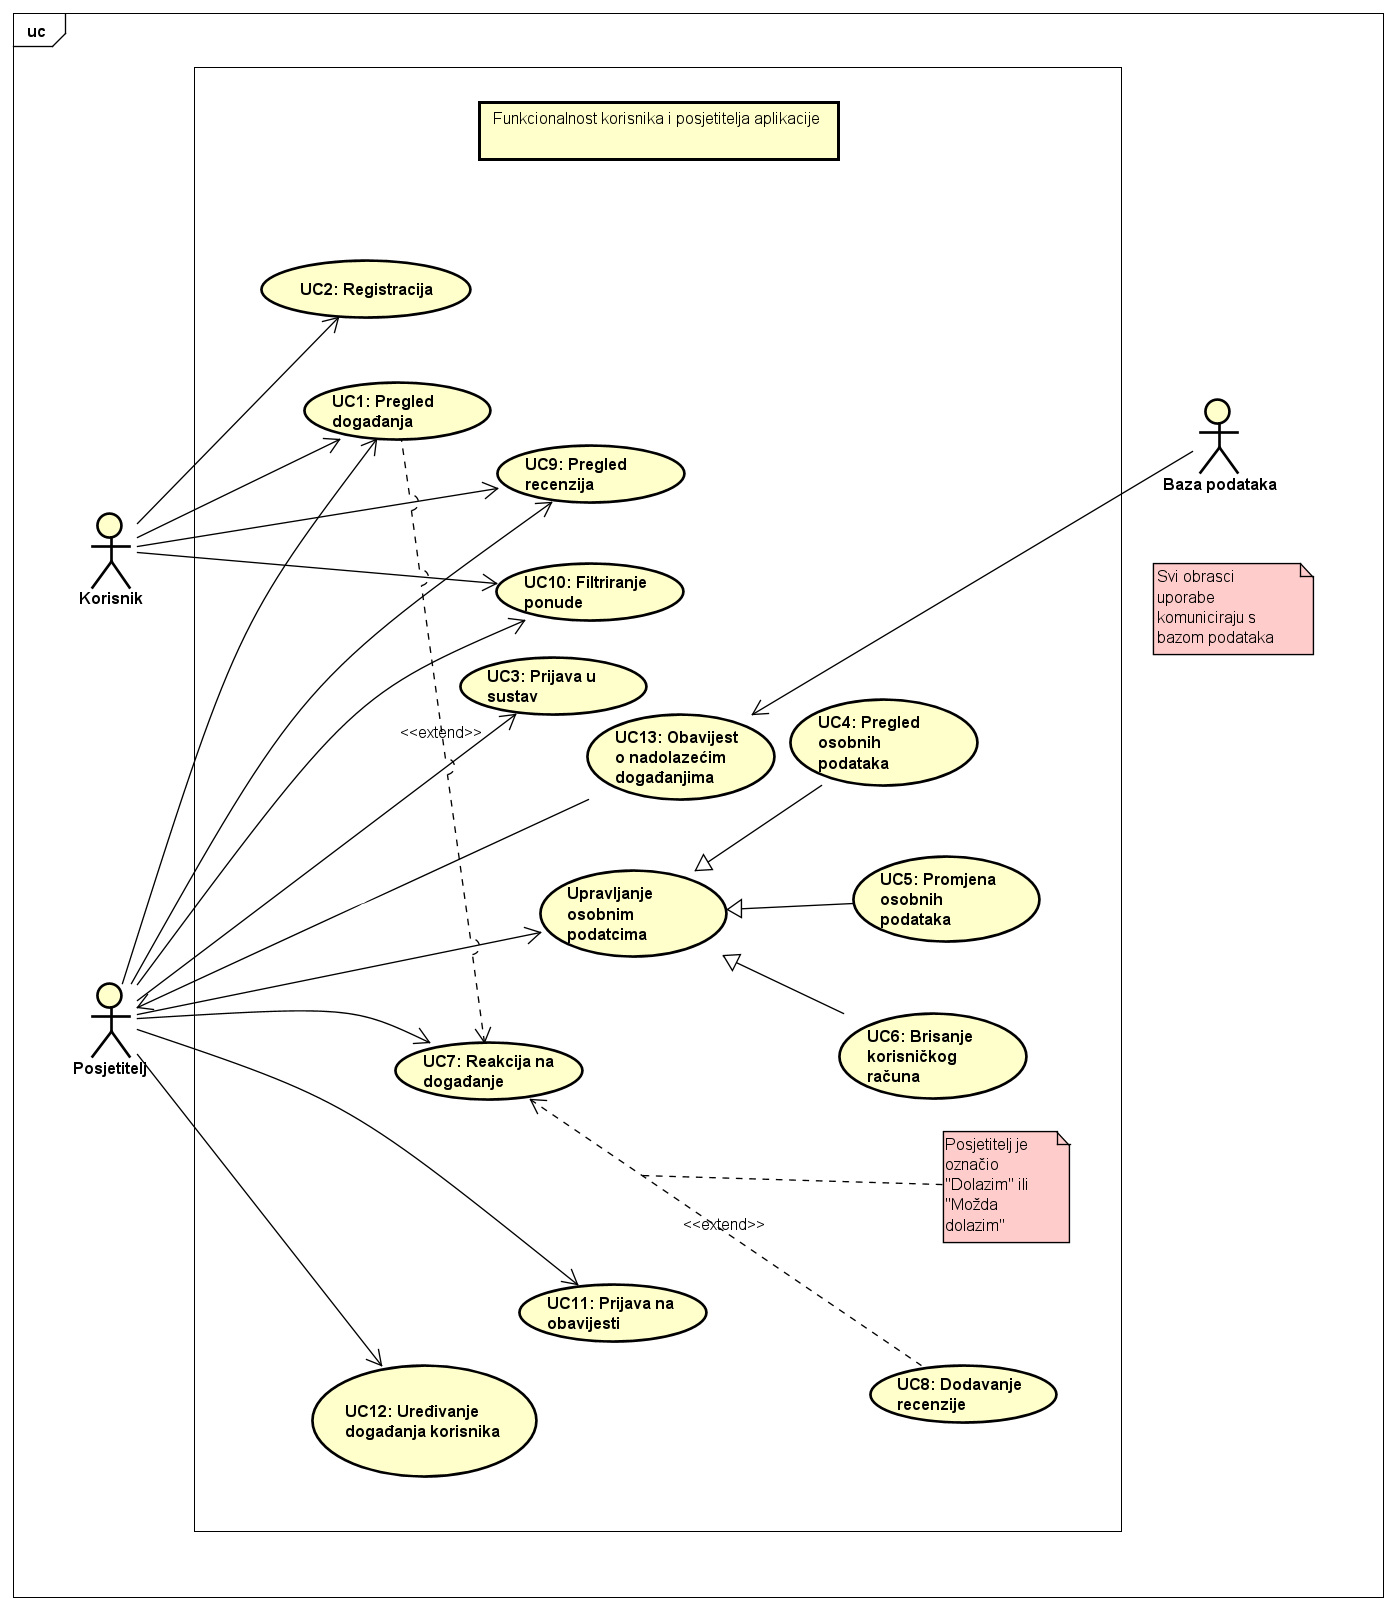
\includegraphics[width=\textwidth]{slike/UCD1-1.PNG}
						\caption{Dijagram obrasca uporabe, funkcionalnost korisnika i posjetitelja}
						\label{fig:UCD1}
					\end{figure}
					
					\begin{figure}[H]
						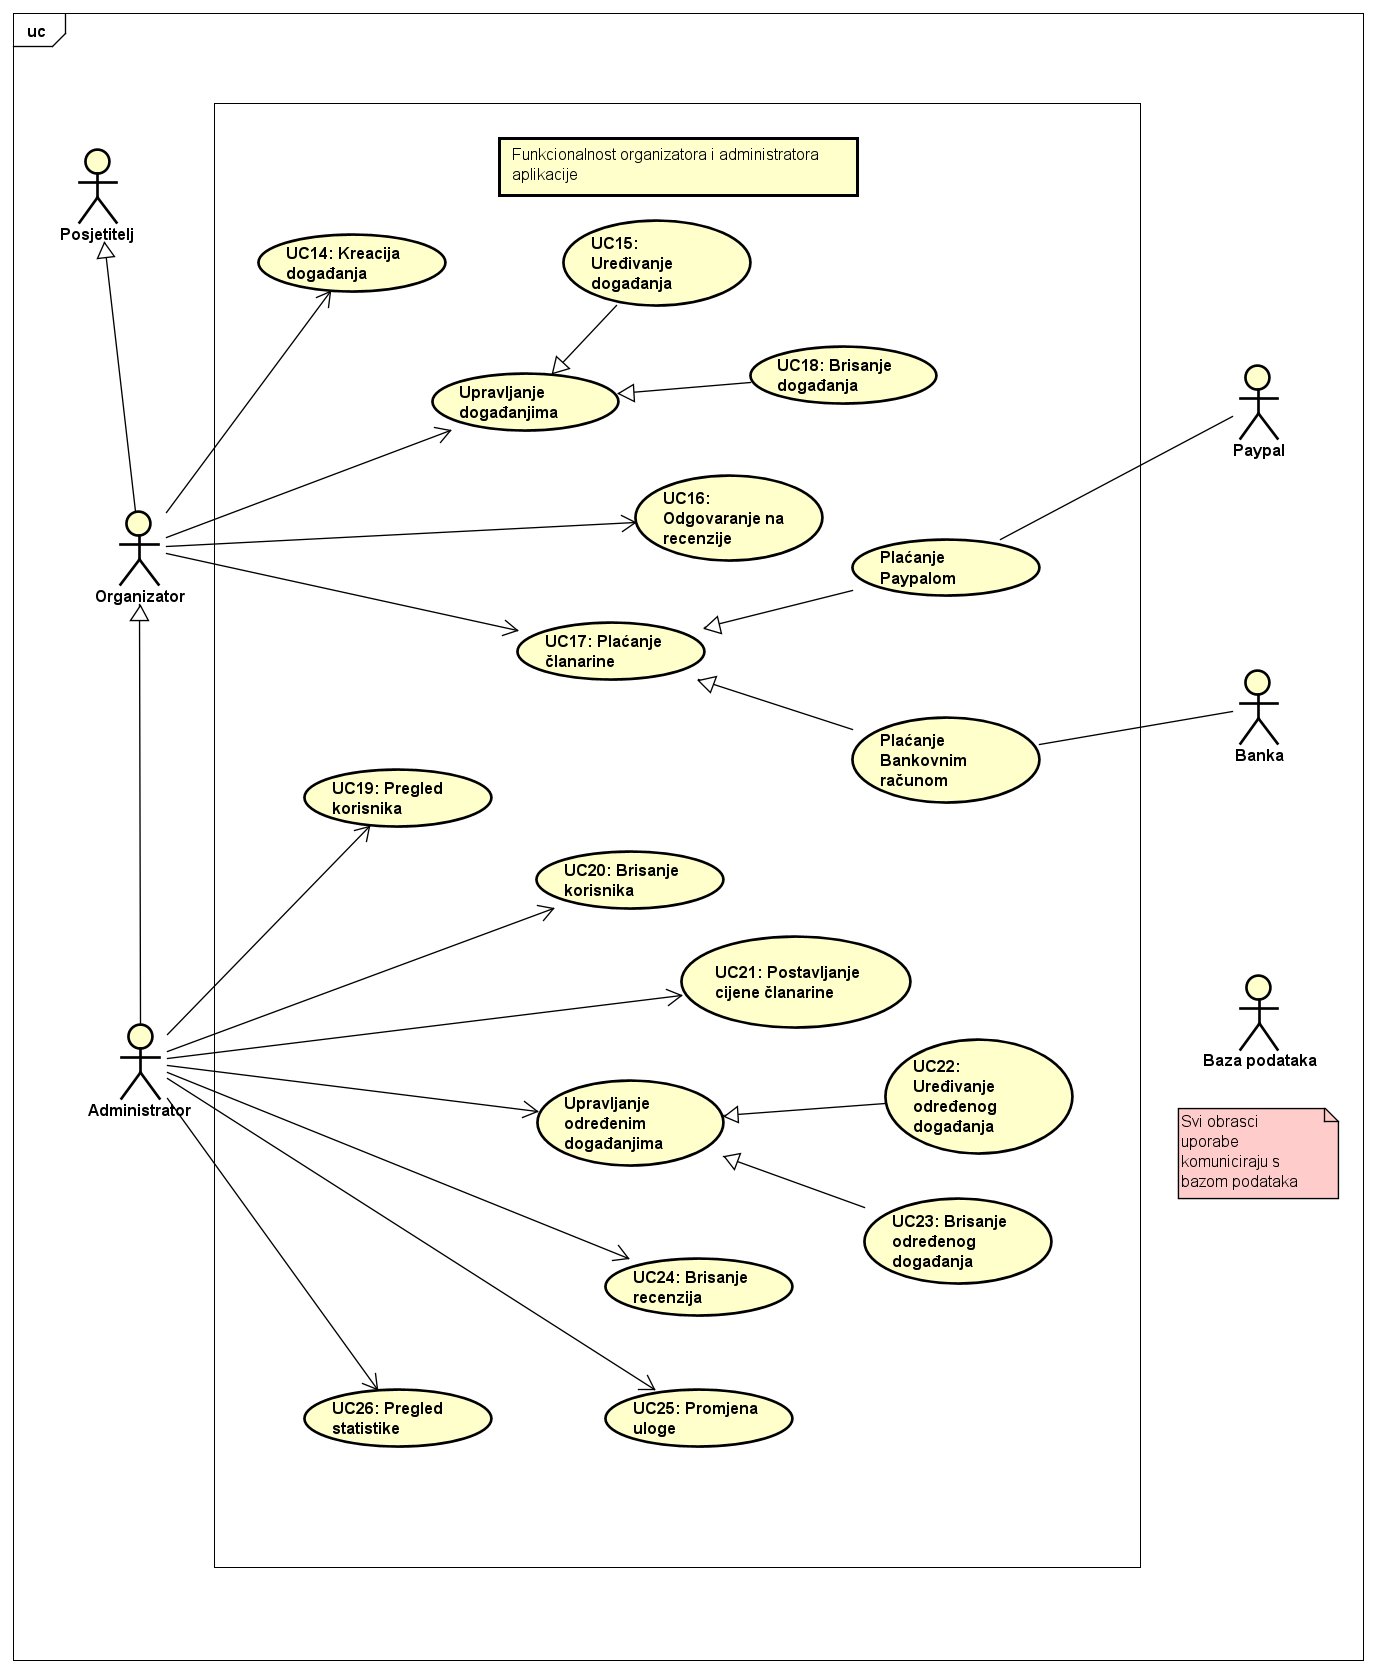
\includegraphics[width=\textwidth]{slike/UCD2-1.PNG}
						\caption{Dijagram obrasca uporabe, funkcionalnost organizatora i administratora}
						\label{fig:UCD2}
					\end{figure}
				\eject		
				
			\subsection{Sekvencijski dijagrami}
				
				%\textbf{\textit{dio 1. revizije}}\\
				
				%\textit{Nacrtati sekvencijske dijagrame koji modeliraju najvažnije dijelove sustava (max. 4 dijagrama). Ukoliko postoji nedoumica oko odabira, razjasniti s asistentom. Uz svaki dijagram napisati detaljni opis dijagrama.}
				
				
				\textbf{\large Obrazac uporabe UC2 - Registracija}\\
				
				
				Klijent odabirom opcije za registraciju šalje zahtjev za prikaz odgovarajuće stranice. Poslužitelj dohvaća tu stranicu i prikazuje ju. Klijent unosi osobne podatke, postavlja lozinku i bira ulogu. Aplikacija provjerava jesu li svi podatci u traženom format i postoji li već takav klijent u sustavu. Ako podatci nisu u zadanom formatu, aplikacija šalje obavijest o tome i klijent iznova unosi potrebne podatke. Ako takav klijent već postoji u sustavu, aplikacija klijentu šalje obavijest o tome. Ako su podatci uneseni u traženom format i takav klijent ne postoji u sustavu, aplikacija u bazu podataka prosljeđuje dobivene podatke, a klijentu šalje obavijest o uspješnoj registraciji.
				\begin{figure}[H]
						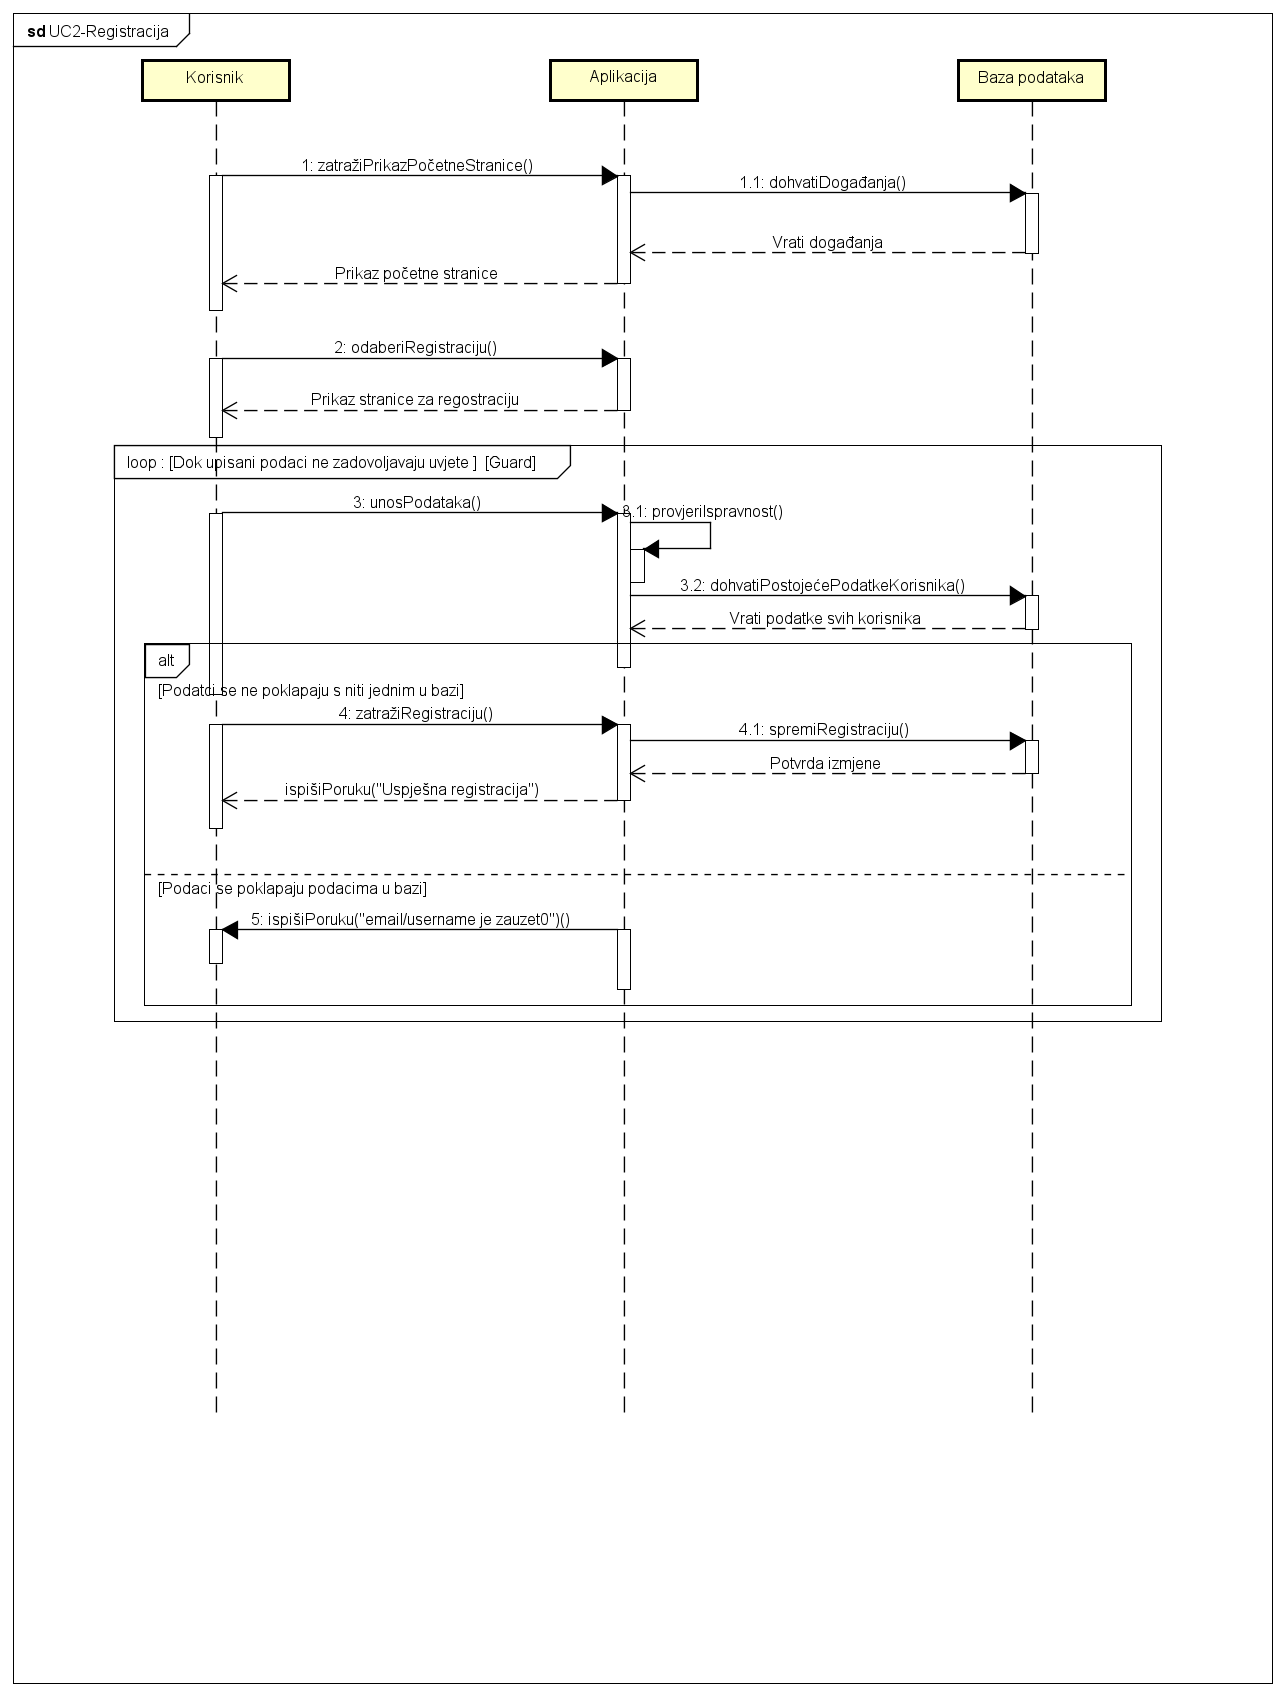
\includegraphics[width=\textwidth]{slike/uc2-1.PNG}
						\caption{Sekvencijski dijagram za UC2}
						\label{fig:uc2}
				\end{figure}
				
				
				\eject
	
				
				
				\textbf{\large Obrazac uporabe UC5 - Promjena osobnih podataka}\\


				Korisnik šalje zahtjev za prikaz stranice za izmjenu podataka. Poslužitelj dohvaća i prikazuje traženu stranicu. Korisnik izmjenjuje svoje podatke i odabire opciju za spremanje podataka. Ukoliko korisnik ne odabere tu opciju, poslužitelj korisniku notifikacijom skreće pozornost na to. Ukoliko podatci ne zadovoljavaju traženi format, aplikacija notifikacijom skreće korisniku pozornost na to. Ukoliko su podatci u traženom formatu, poslužitelj ih ažurira u bazi podataka.
				\begin{figure}[H]
						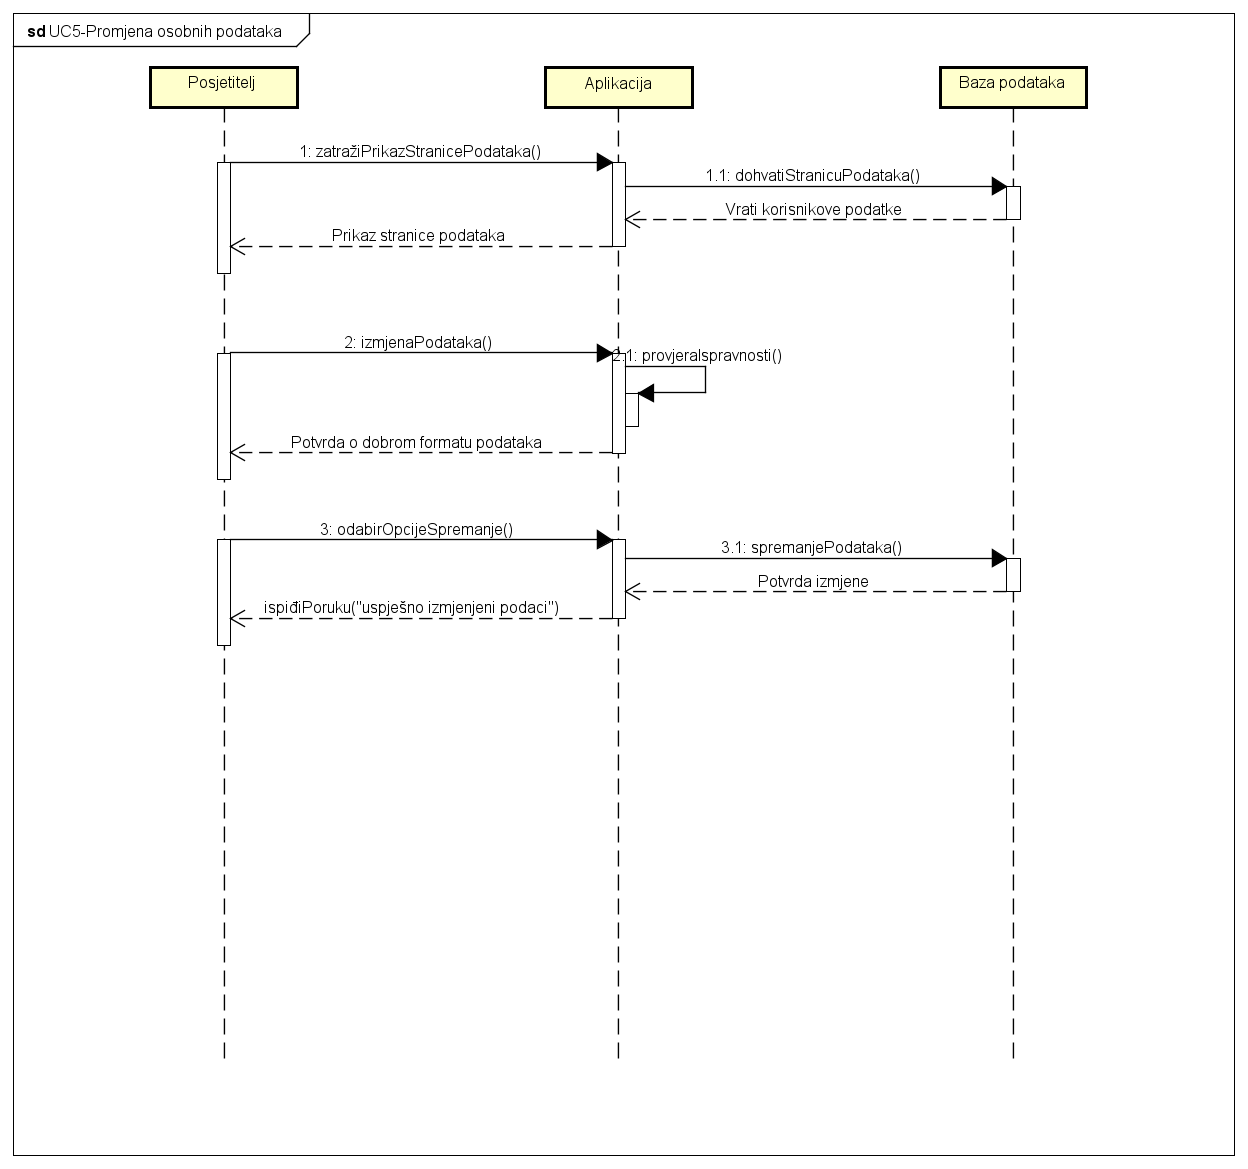
\includegraphics[width=\textwidth]{slike/uc5-1.PNG} 
						\caption{Sekvencijski dijagram za UC5}
						\label{fig:uc5}
				\end{figure}

				
				\eject
				
				
				
				\textbf{\large Obrazac uporabe UC14 - Kreacija događanja}\\
				
				Klijent poslužitelju šalje zahtjev za prikaz stranice za kreiranje novog događanja. Poslužitelj dohvaća traženu stranicu i prikazuje ju. Klijent unosi podatke i fotografije, a po izboru i cijenu ulaznice. Ako je klijent postavio cijenu događanja, poslužitelj dohvaća podatke o klijentu iz baze podataka i provjerava jeli uplatio članarinu. Ako nije, poslužitelj ga o tome obavještava notifikacijom i klijent prihvaća ili odbija pretplatiti se. Ako se pretplati, poslužitelj unosi događanje u bazu podataka. Ako klijent ne postavi cijenu događanja, poslužitelj nista ne provjerava i sprema podatke o događanju u bazu podataka.
				
				\begin{figure}[H]
						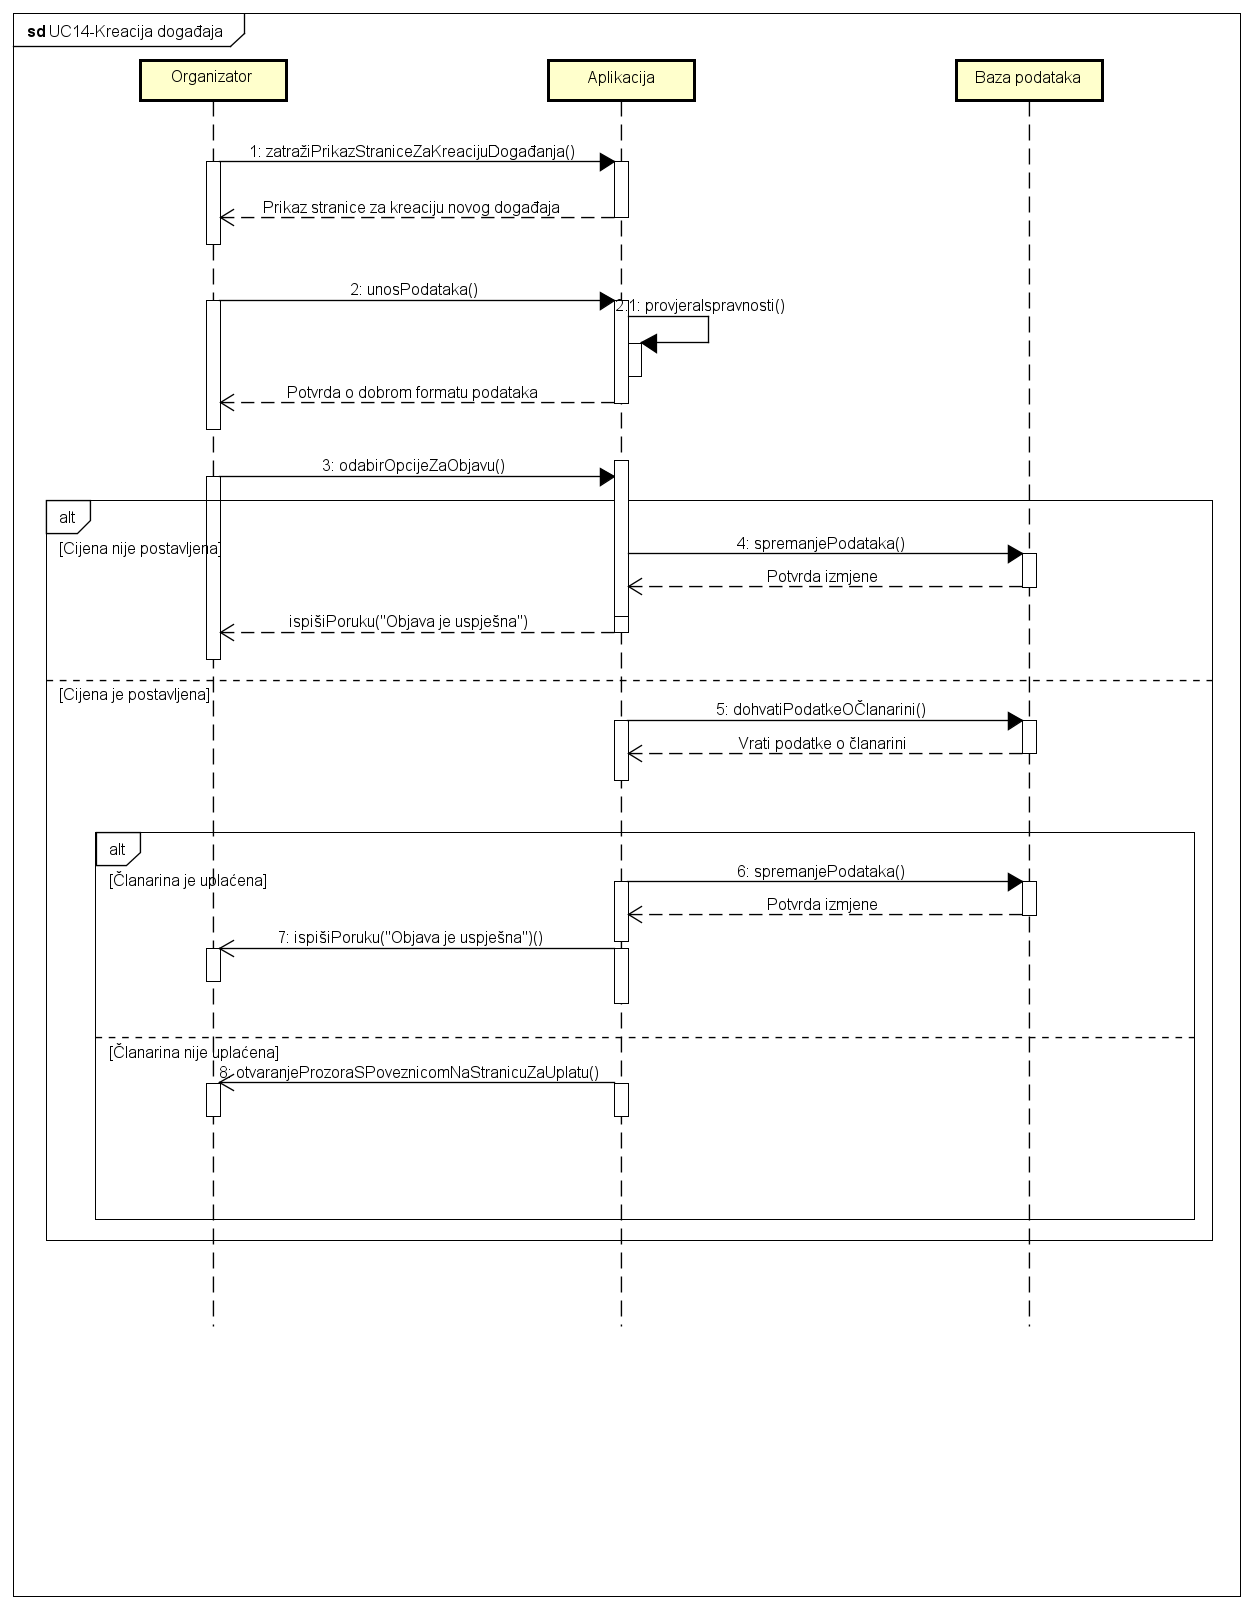
\includegraphics[width=\textwidth]{slike/uc14-1.PNG}
						\caption{Sekvencijski dijagram za UC14}
						\label{fig:uc14}
				\end{figure}
				
				\eject
				
				
				\textbf{\large Obrazac uporabe UC20 - Brisanje korisnika}\\
				
				Administrator odabire opciju za prikaz stranice za pregled korisnika. Poslužitelj dohvaća stranicu i prikazuje ju administratoru. Administrator odabire korisnika kojeg treba izbrisati. Potvrđuje svoj odabir i time šalje zahtjev za brisanjem poslužitelju. Poslužitelj dohvaća bazu podataka i iz nje uklanja podatke o korisniku i samog korisnika. Administratoru šalje obavijest o uspješnom brisanju.
				
				\begin{figure}[H]
						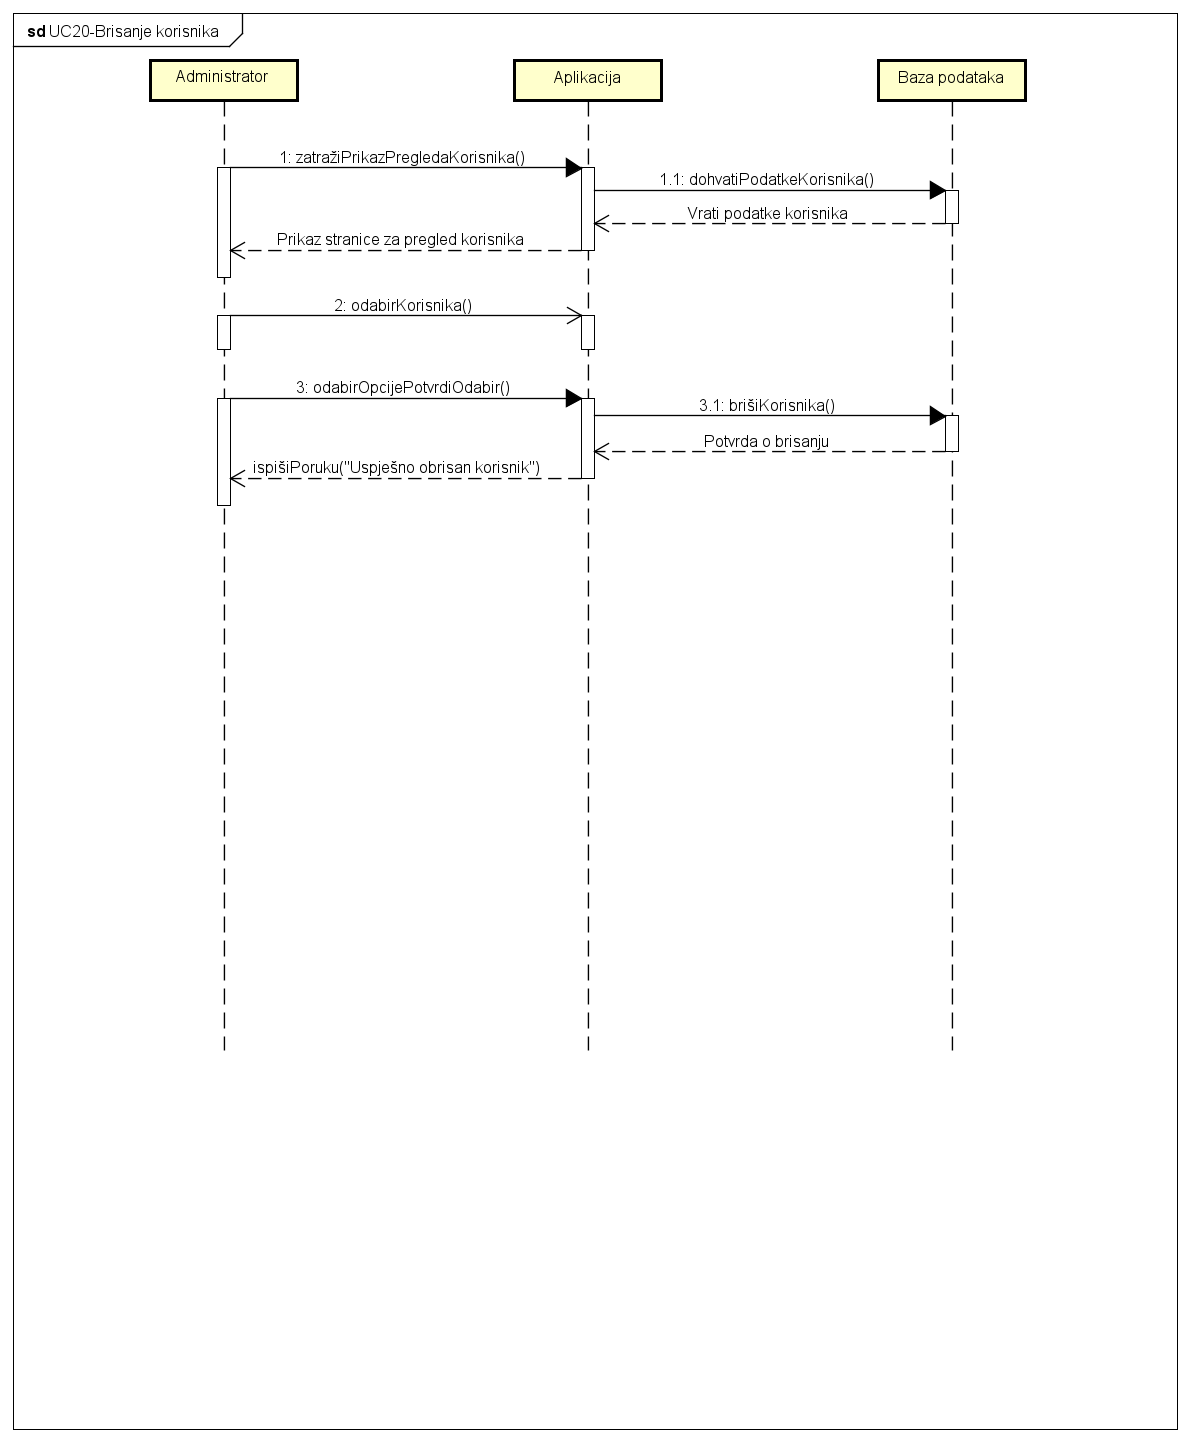
\includegraphics[width=\textwidth]{slike/uc20-1.PNG} 
						\caption{Sekvencijski dijagram za UC20}
						\label{fig:uc20}
				\end{figure}

				\eject
	
		\section{Ostali zahtjevi}
		
			\begin{packed_item}
	
						\item Sustav treba omogućiti rad više korisnika od jednom u stvarnom vremenu
						\item Korisničko sučelje i sustav moraju podržavati hrvatsku abecedu (dijakritičke znakove) pri unosu i prikazu tekstualnog sadržaja
						
						\item Izvršavanje dijela programa u kojem se pristupa bazi podataka ne smije trajati duže od nekoliko sekundi
						
						\item Sustav treba biti implementiran kao web aplikacija koristeći objektno-orijentirane jezike
						
						\item Neispravno korištenje korisničkog sučelja ne smije narušiti funkcionalnost i rad sustava
						
						\item Sustav treba biti jednostavan za korištenje, korisnici se moraju znati koristiti sučeljem bez opširnih uputa
						
						\item Nadogradnja sustava ne smije narušavati postojeće funkcionalnosti sustava
						
						\item Sustav kao valutu koristi EUR
						
						\item Veza s bazom podataka mora biti kvalitetno zaštićena, brza i otporna na vanjske greške
						
						\item Pristup sustavu mora biti omogućen iz javne mreže pomoću HTTPS
						\item Sučelje mora biti estetski privlačno
						
					
						
						
						
			\end{packed_item}
			
			 
	